\documentclass[paper=a4paper,jafontsize=9pt,head_space=15mm,gutter=20mm,
twocolumn,number_of_lines=49, line_length=26zw]{myuarticle}

\begin{document}

\title{{\Large\bfseries\gtfamily 環境情報のセンシングを用いた他者の環境評価を表現するロボットシステム}}
\author{\\\ 22120165 中村龍造 \\ (指導教員 : 佐藤宏樹)\\ \\}
\date{}
\maketitle

\section{はじめに}
生活空間には,人間以外にも多くの存在が共存している.それらの存在は,それぞれ独自の感覚や基準で環境を捉えているが,その感覚を直接共有することはできない.このような「他者」の経験を理解し,共感することは,多様な存在との共生を考える上で重要な課題となっている.

本稿では,取得した環境データに対して,人間,動植物,非生物などといった複数の他者からの評価基準を設定し,評価結果をロボットの身体的動作を通して表現するシステム(以下「本システム」)を提案する.本システムを通じて,ユーザーが他者にとっての快適さを知り,他者への理解,関心を深めることで,多様な存在との対話の機会創出を目指す.

\section{関連研究と課題}

他者視点の表現に関する取り組みとしては,In the Eyes of the Animal\cite{Dezeen-2015-MarshmallowLaserFeastsEyes}のようなVRによる体験の共有や,rapoptosis\cite{--ソンヨン}のようなモノの自立的な意思決定の表現が提案されている.しかしこれらの手法は一時的な体験や特定の対象に限定されており,生活空間における継続的な他者視点の理解を支援することは難しい.

人間を対象とした場合でも,環境への評価は個々人で差異があり,客観的指標による評価のみならず,主観での評価を取り入れる必要があると言われている\cite{Coulby-2020-ScopingReviewTechnologicalApproaches}.

\section{システム要件}

上記の課題を踏まえ,本研究では人間,動植物,非生物など,様々な他者を基準に,それらから見た環境の快・不快をロボットの身体的動作で表現するシステムを開発する.ロボットという物理的な存在を用いることで,生活空間における他者の視点を継続的に表現し,共生への理解を深めることを目指す.

このような目的を達成するため,本システムの開発にあたって以下の3点を要件とする:

\begin{description}
  \item[継続的な表現:] 生活空間において,ロボットが常に存在し続けることで,環境変化に応じた他者の評価を途切れることなく表現できること
  \item[多様な他者の表現:] 人間,動植物,非生物など様々な他者の環境評価基準を設定し,それぞれの特徴を反映した動作で表現できること
  \item[日常的な理解支援:] ユーザーが特別な操作をすることなく,生活空間における他者との環境認識の違いを自然に理解できること
\end{description}

\subsection{全体のフロー}
本システムは,ユーザー,環境,センサー,ロボット,本システムの5つからなる.システム全体のフローを図\ref{fig:system-flow}に示す.

\fboxsep=0pt            %画像と枠線をくっつける.
\fboxrule=1pt            %枠線の太さを1ptにする.
\begin{figure}[h]
  \centering
  \fbox{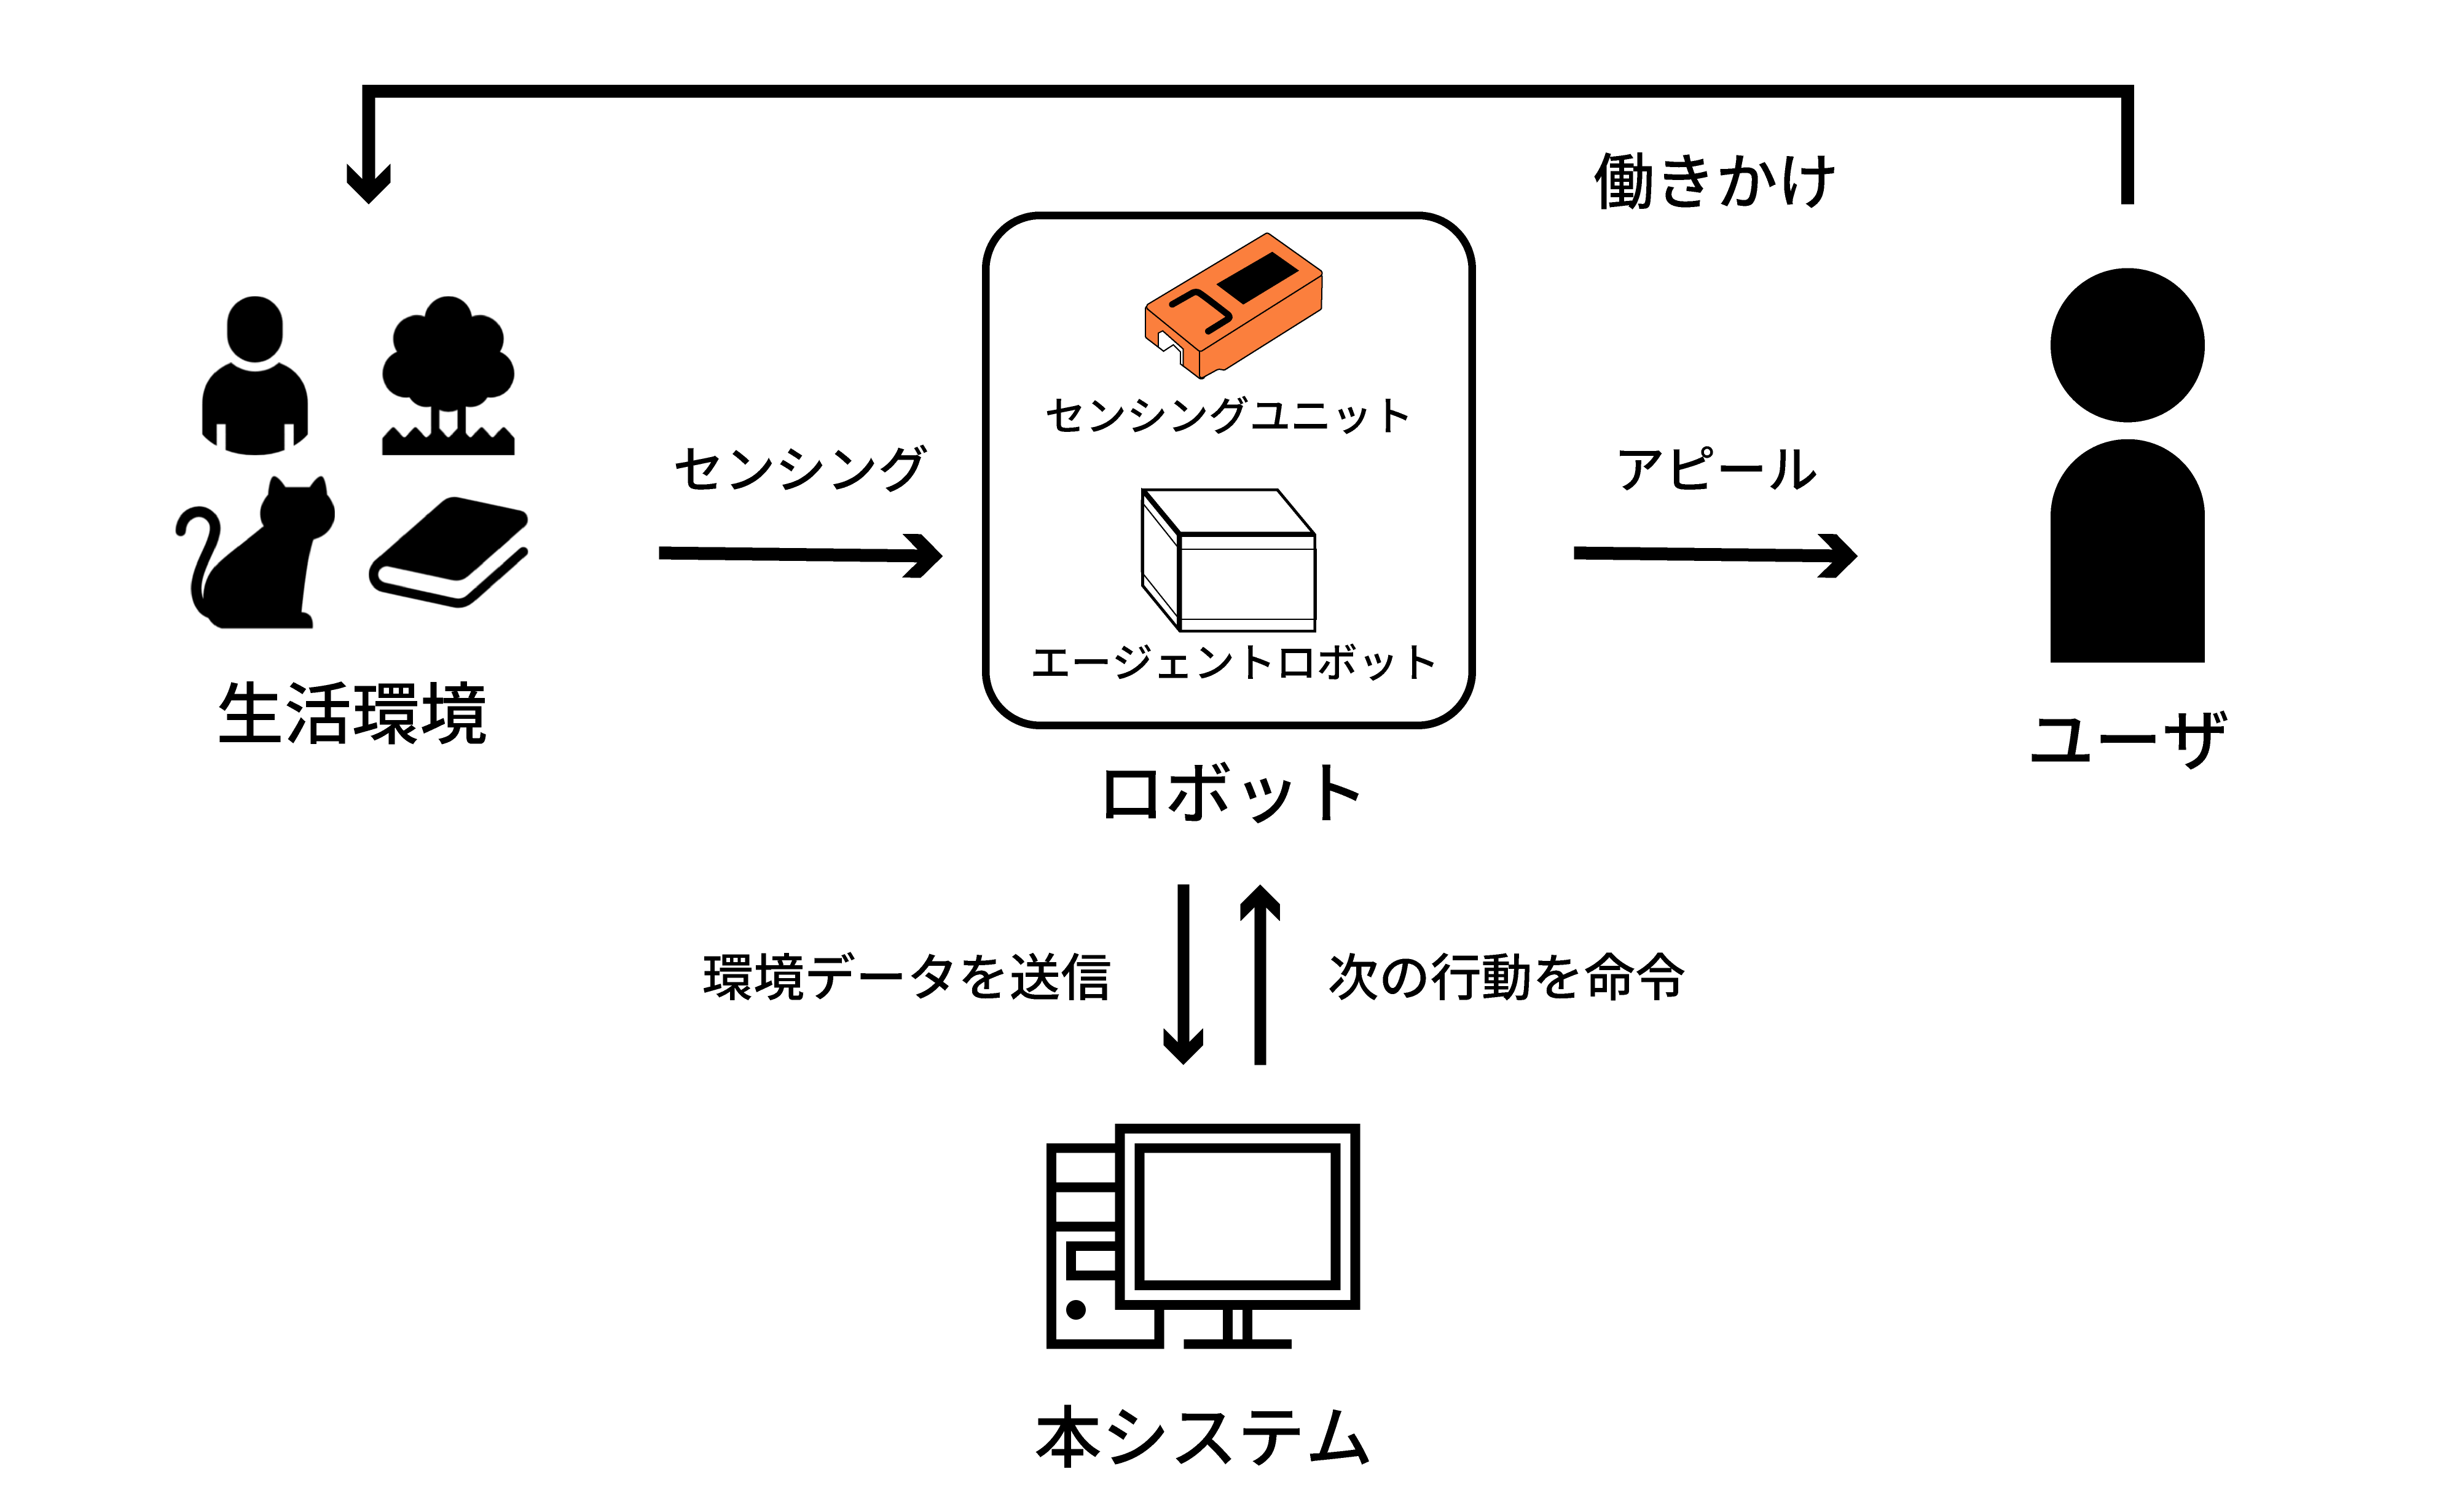
\includegraphics[keepaspectratio, clip,
  width=0.8\columnwidth]{resources/system_flow.png}}
  \caption{システム全体のフロー図}
  \label{fig:system-flow}
\end{figure}

はじめに本システムが,センサーを通じて生活空間の環境データを取得する.他者を基準とした評価,評価に応じて快・不快をアピールするなどの行動命令を現実空間のロボットに送信する.ロボットは行動命令に従って人間にアピールする.それを見た人間が環境や他者に対して働きかけることで,他者にとってより快適な環境を得る.

\section{本システムの実装}
本システムは,センシングシステム,評価システム,アクション生成システム,ロボット制御システムから構成される.ハードウェアは,センシングデバイスにM5StickC(M5Stack社)を,ロボットにtoio(SONY社)を用いた.

本システムでは,各主体(人間,動物,物体など)について,その対象にとって最適な環境条件を設定し,現在の環境がその条件からどの程度離れているかに応じてロボットの動作を変化させる.

これらの条件に基づき、環境センサーから得られた測定値と最適条件との差異を評価し、ロボットの動作を決定する。

本システムの構造を図\ref{fig:system-structure}に示す.

\fboxsep=0pt            %画像と枠線をくっつける.
\fboxrule=1pt            %枠線の太さを1ptにする.
\begin{figure}[h]
  \centering
  \fbox{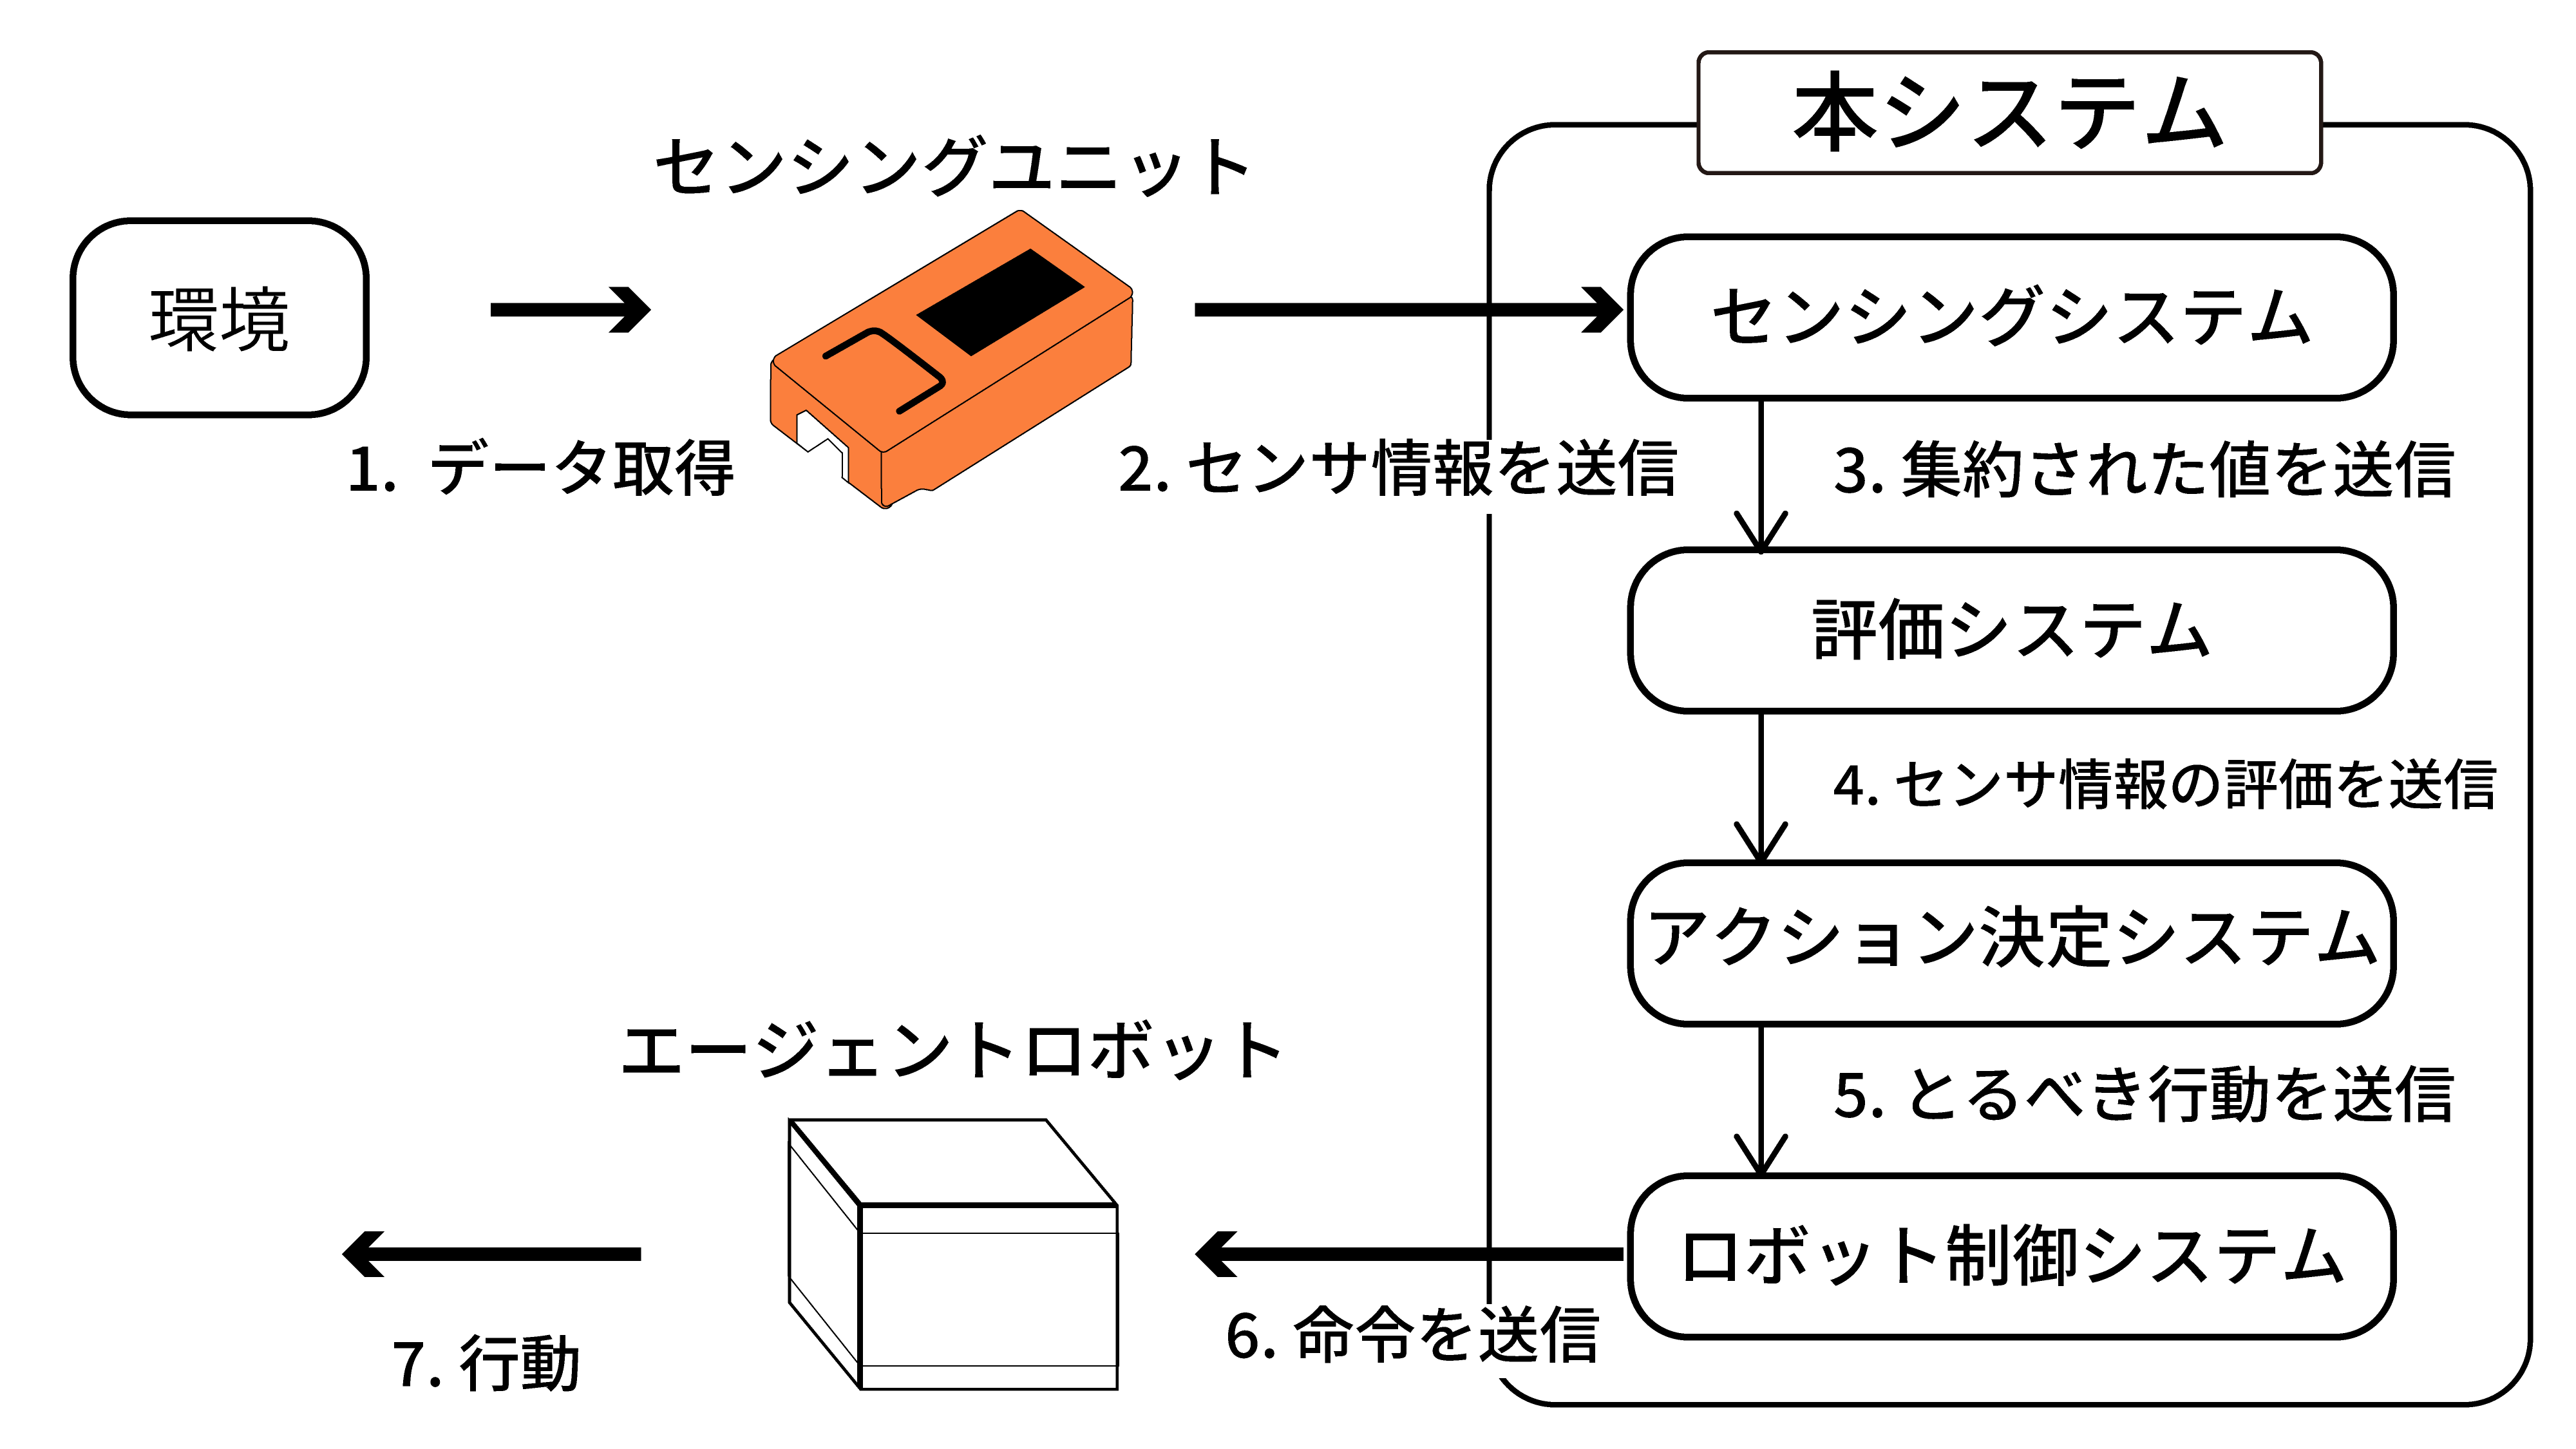
\includegraphics[keepaspectratio, clip,
  width=0.8\columnwidth]{resources/system_structure.png}}
  \caption{本システムの構造図}
  \label{fig:system-structure}
\end{figure}

\subsection{センシングシステム}

センシングシステムは,センサーから送信されたデータを受け取り,以後のシステムにデータを提供する.

\subsection{評価システム}
評価システムでは,センサーシステムから環境データを取得・評価し,評価データを生成する.評価データは,環境データと評価基準値との差をスコアとして所持している.対象データの評価では,例えば人間に適した気温であれば18~24℃などと,あらかじめ対象データの主体にとって最適な範囲を設定する.現在の気温が最適範囲から外れた場合,上回れば正の,下回れば負のスコアをもった評価データを生成する.システム開発者は評価主体とその評価対象ごとに,個別の評価システムを実装する必要がある.

\subsection{アクション生成システム}
アクション生成システムでは,評価システムから取得した評価データをもとに,評価に応じたアクション命令をロボット制御システムへ送る.アクション開発者は,主体および対象の環境データごとにアクションを作成しておく必要がある.本システムのアクションは,岡田ら\cite{岡田-2017-弱いロボ}の「弱いロボット」の概念を取り入れてデザインした.「弱いロボット」は,人間の介入や支援を引き出す手法として「よたよた」とした動きを用いている.本システムでも,この考え方に基づき,環境が快適でない場合のアクションとして,直線的に移動せず,わずかに蛇行しながら進んだり,時折立ち止まったりする動きを実装した.このような不安定な動きによって,ロボットが困っているような印象を与え,ユーザーが環境を確認し,調整するきっかけとなることを期待している.

アクションは「コマンド」のキューで構成される.コマンドはロボット動作用のより低レベルな命令と,動作の所要時間を所持しており,一連のコマンドを実行することで,1つの意味あるアクションを表現する.

\subsection{ロボット制御システム}
ロボット制御システムでは,実機toioとシステム上のtoioを識別するためのデータ管理および,アクション生成システムから取得したアクションの実行を行う.

\section{システムの動作検証}
本システムによってロボットが動作している様子を図\ref{tab:theme-test}に示す.

今回の検証では,以下の3つの主体とその最適環境条件を設定した:
\begin{itemize}
  \item 人間の気温評価:18~28℃\cite{JianZhuWuHuanJingWeiShengGuanLiJiZhunnituite|HouShengLaoDongSheng}
  \item 猫の気温評価:30~38℃\cite{stellaEnvironmentalAspectsDomestic2016}
  \item バナナの保存環境評価:気温14~20℃\cite{--バナナの},湿度45~85\%\cite{--JISZ87031983試験}(生育状態ではなく,室内での食品保存条件として設定)
\end{itemize}

\begin{figure*}[t]
  \centering
  \label{tab:theme-test}
  \begin{tabular}{|c|c|c|c|}
    \hline
    & \sffamily 人間の気温評価 & \sffamily 猫の気温評価 & \sffamily バナナの保存環境評価 \\
    \hline
    快適 &
    \begin{minipage}[c]{0.15\textwidth}
      \centering
      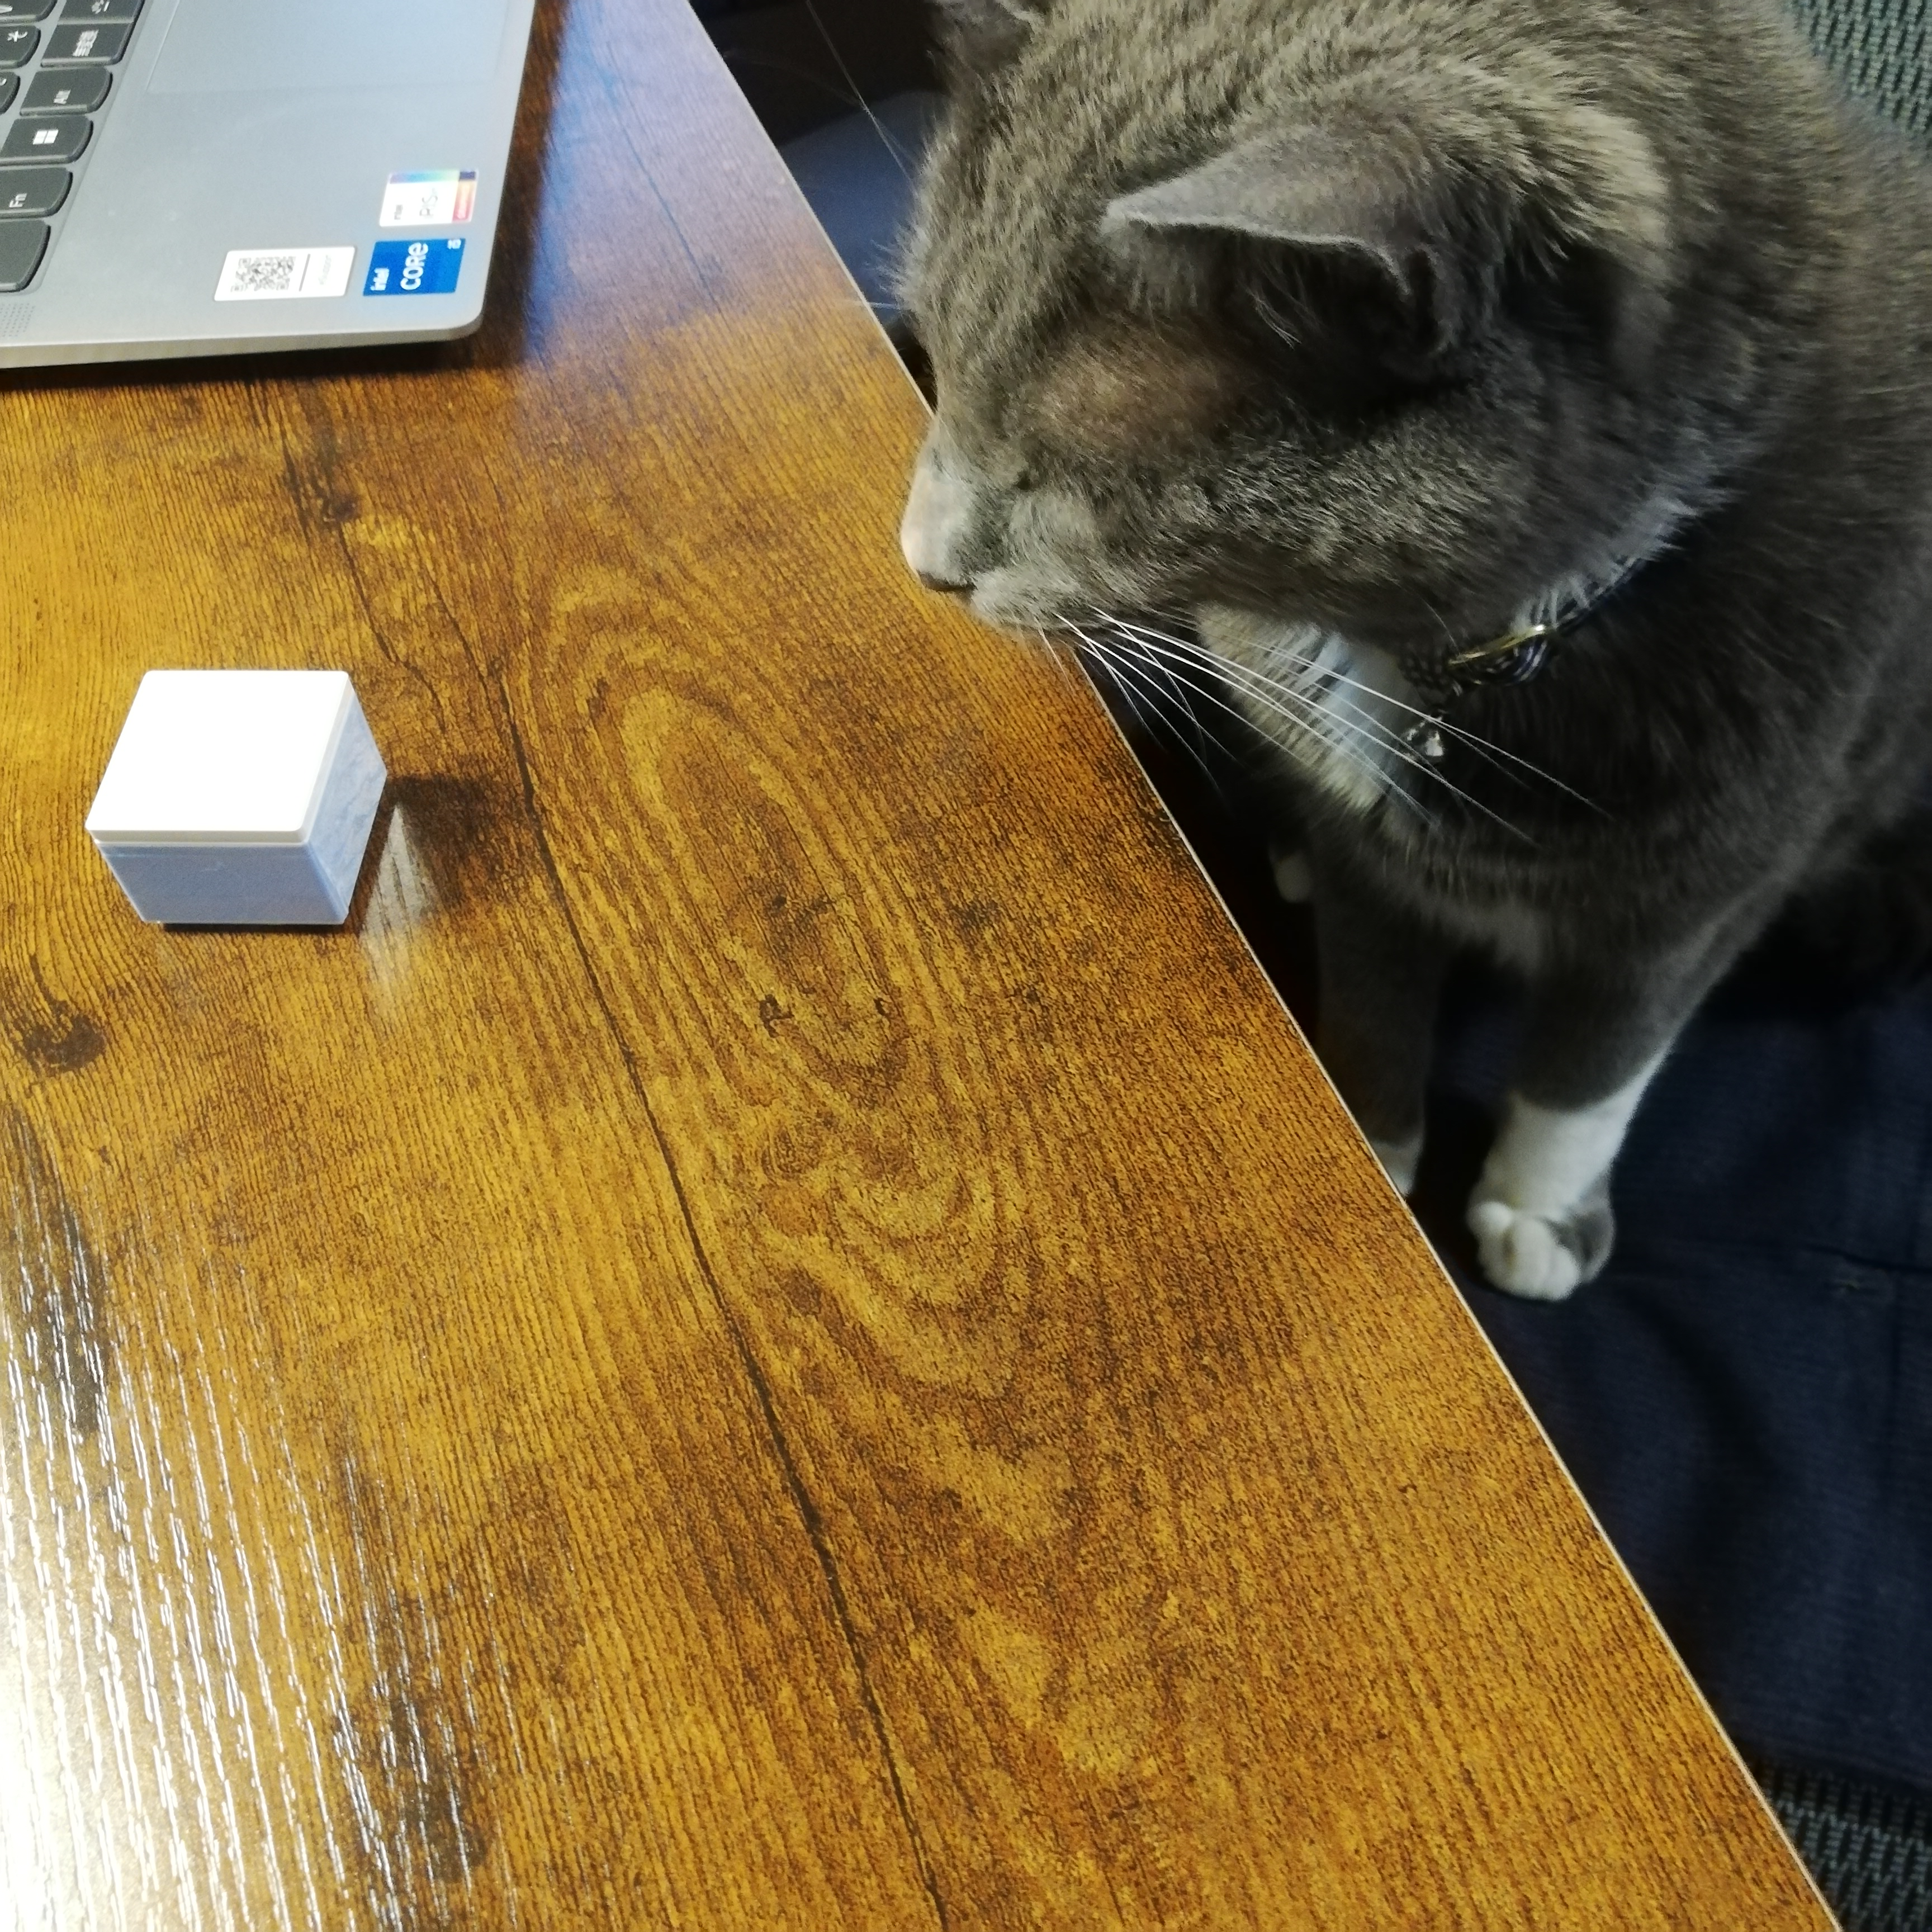
\includegraphics[width=0.9\textwidth]{resources/cat_before.jpg}
    \end{minipage}    &
    \begin{minipage}[c]{0.15\textwidth}
      \centering
      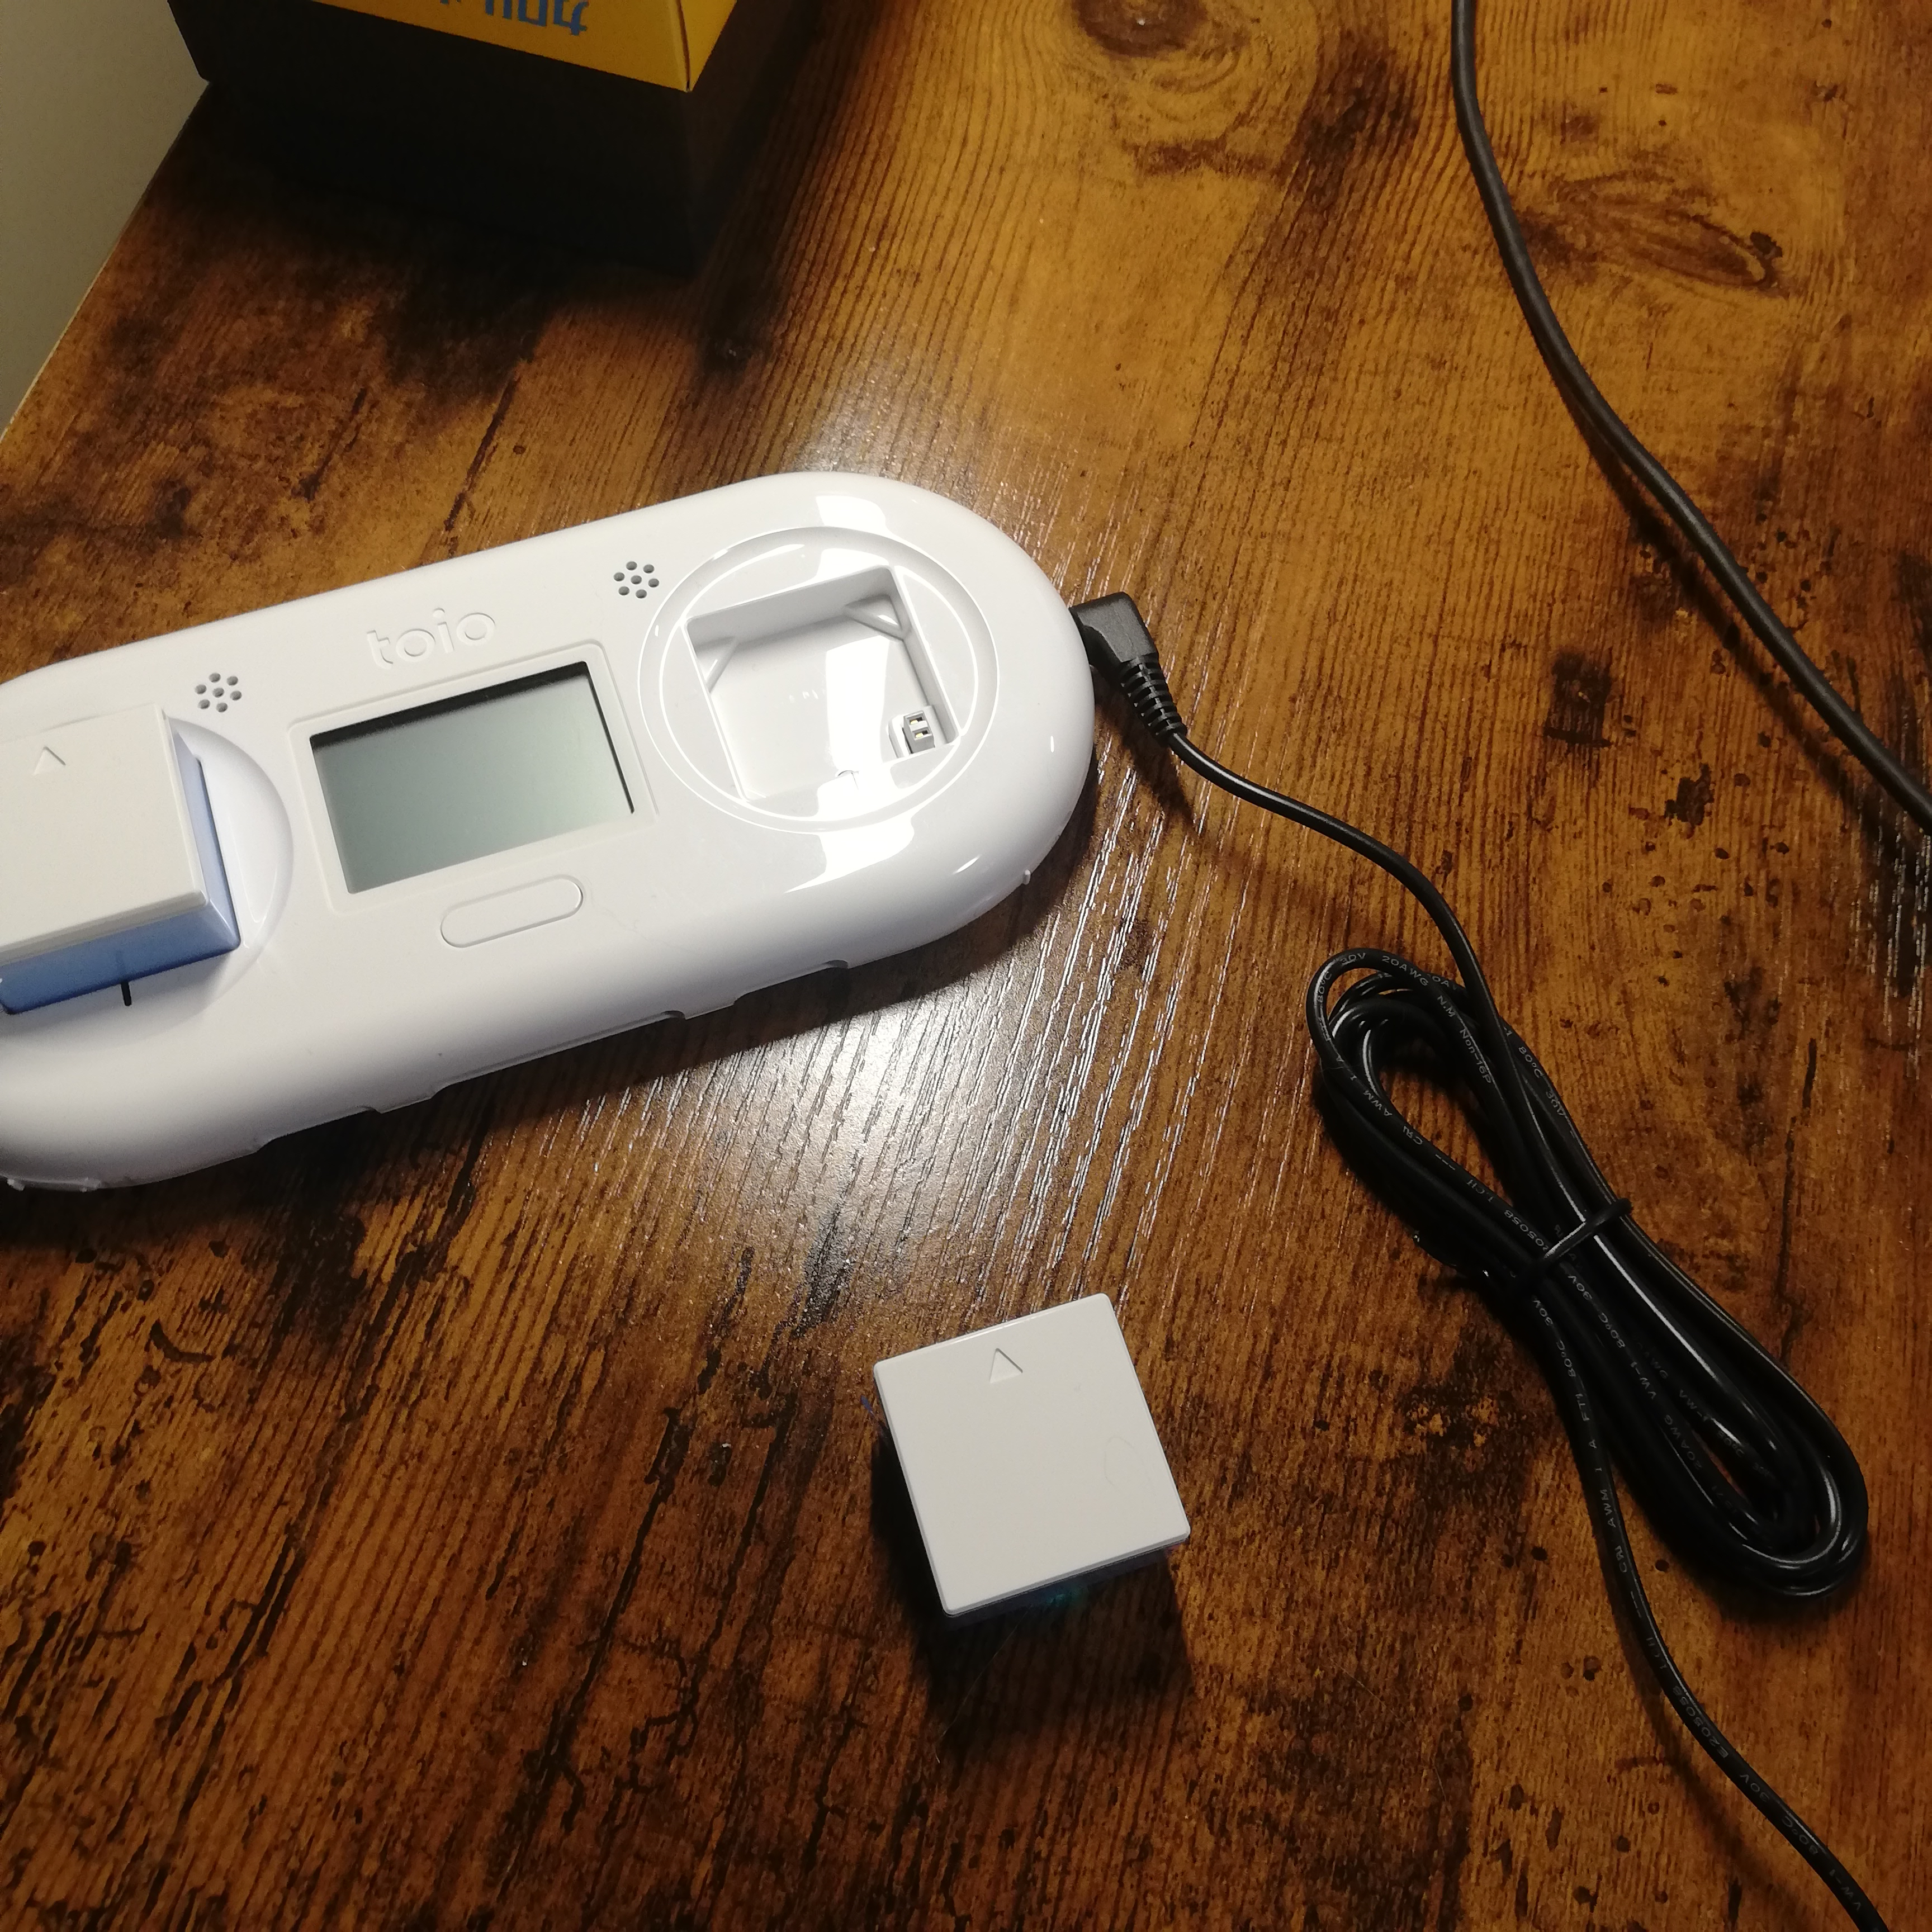
\includegraphics[width=0.9\textwidth]{resources/doc_before.jpg}
    \end{minipage}    &
    \begin{minipage}[c]{0.15\textwidth}
      \centering
      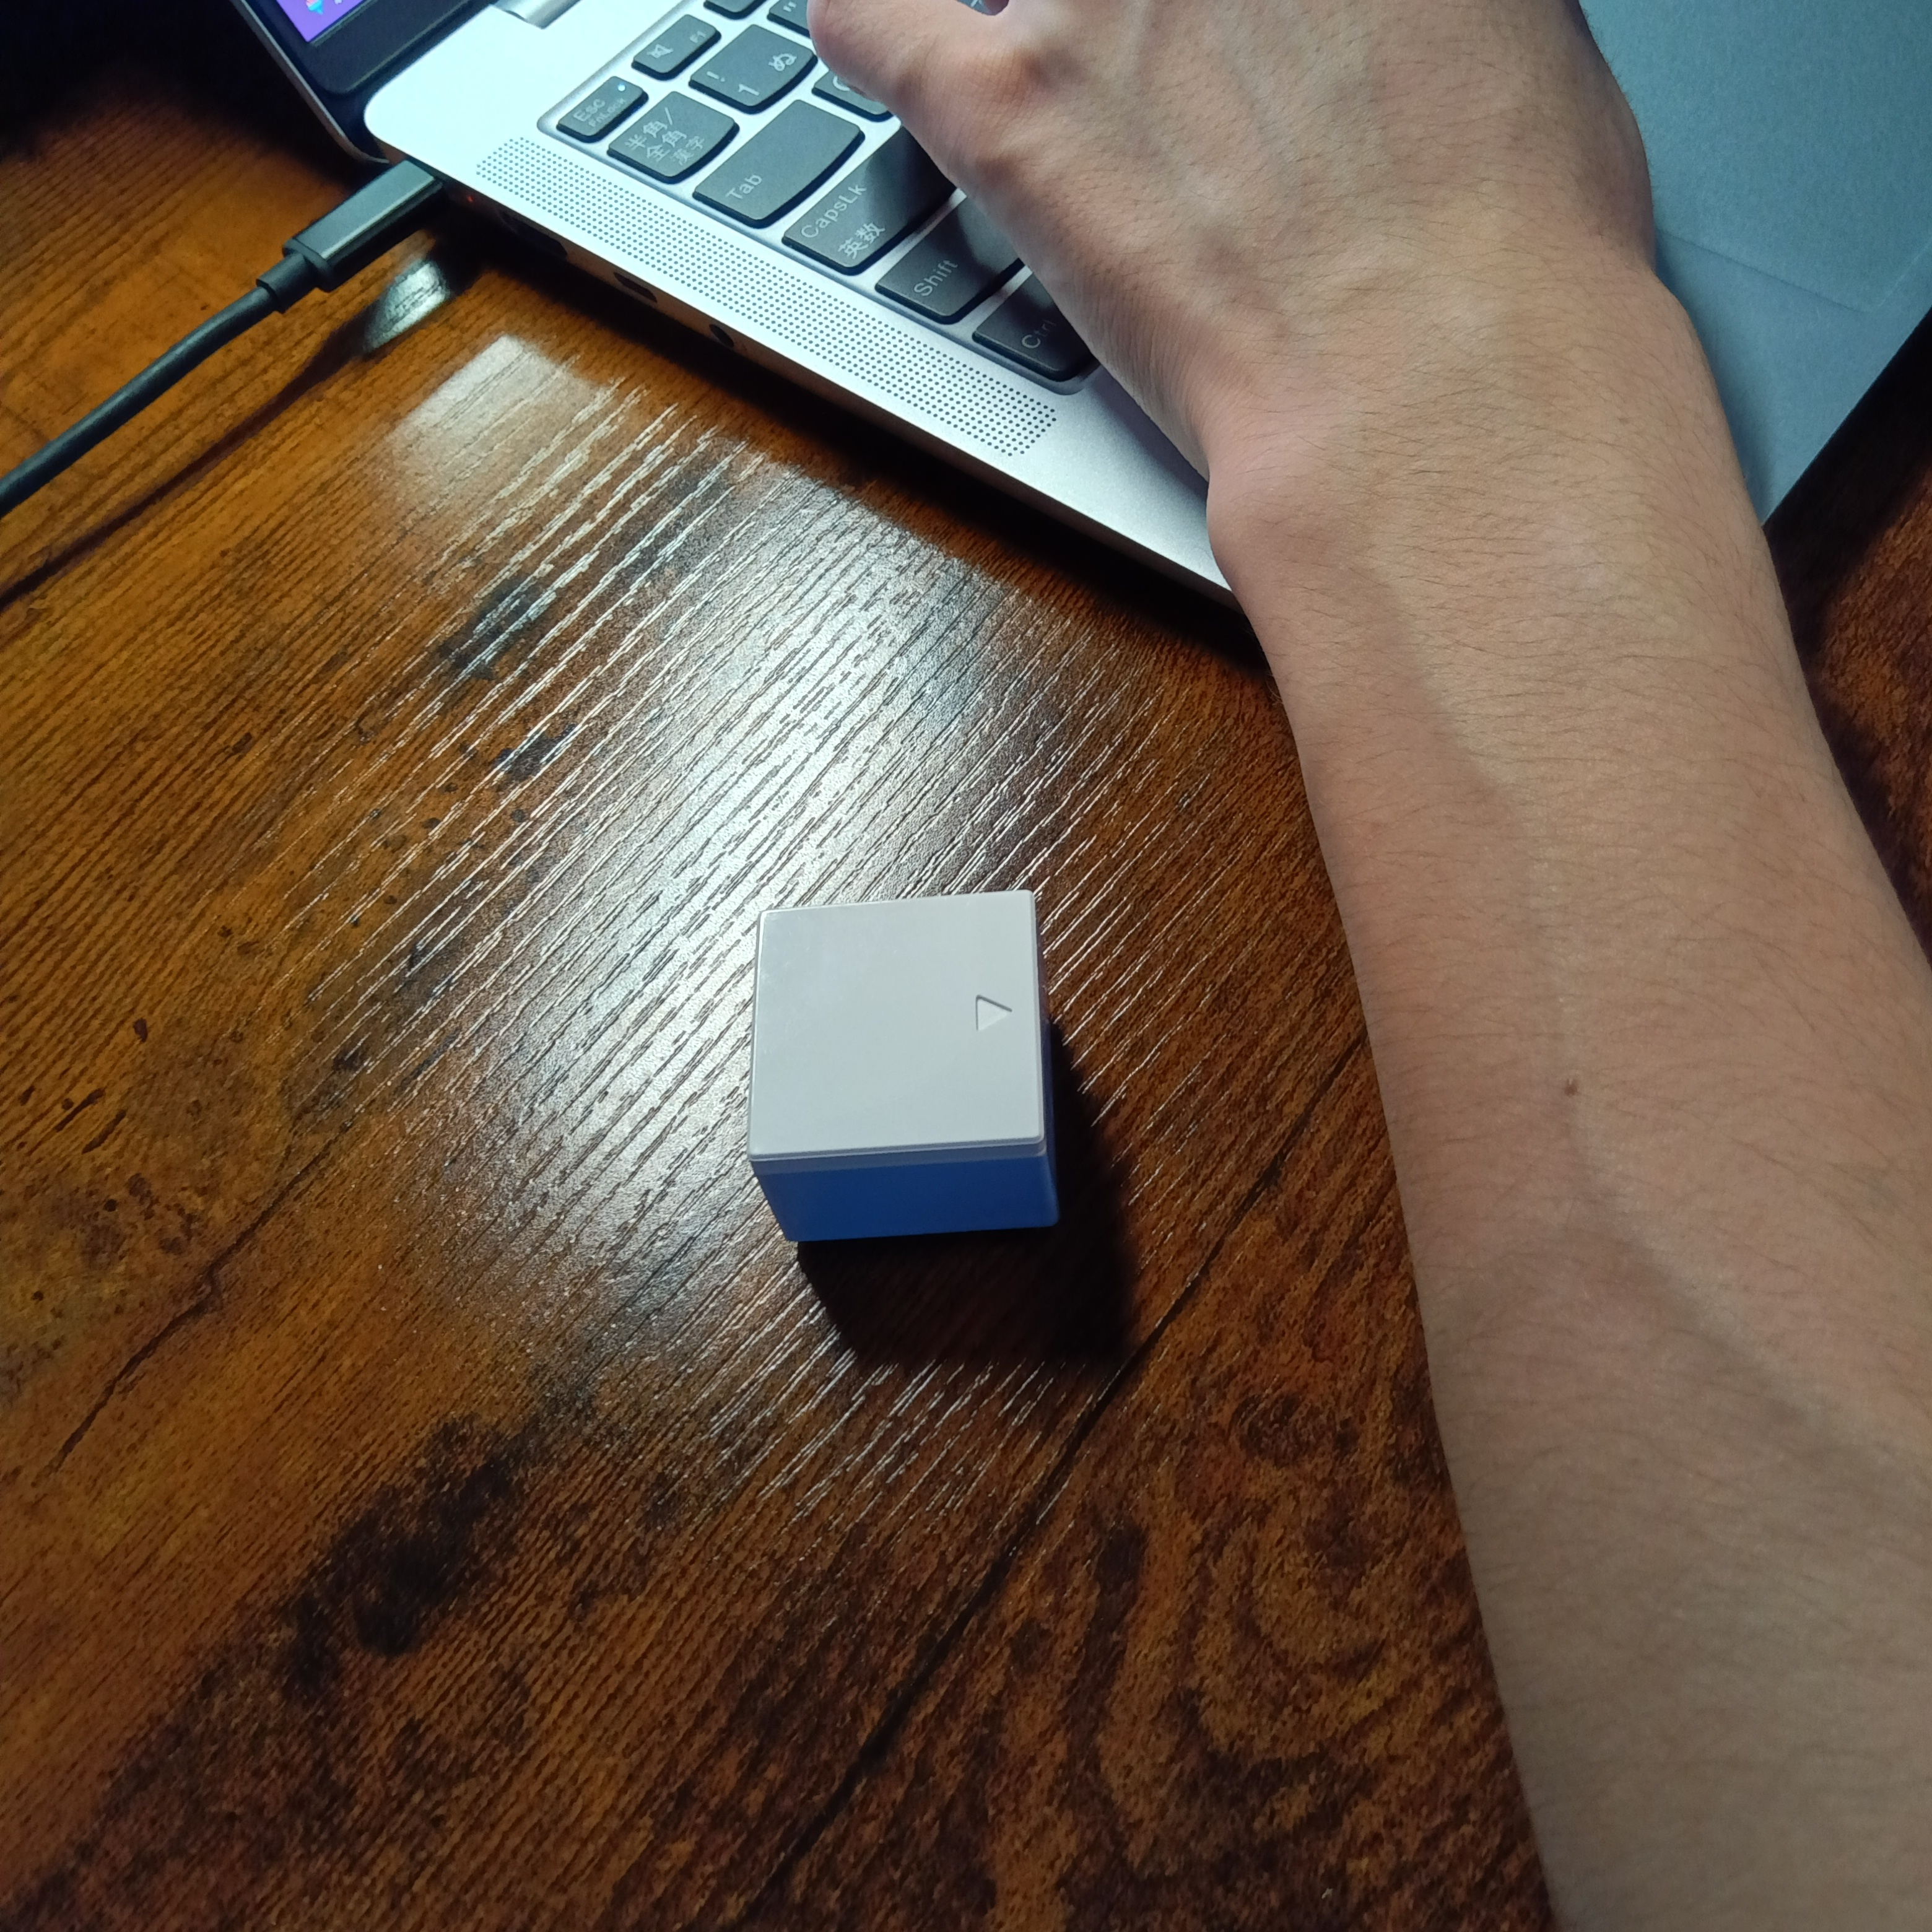
\includegraphics[width=0.9\textwidth]{resources/pet_before.jpg}
    \end{minipage}
    \\ \hline
    % 3行目
    不快 &
    \begin{minipage}[c]{0.15\textwidth}
      \centering
      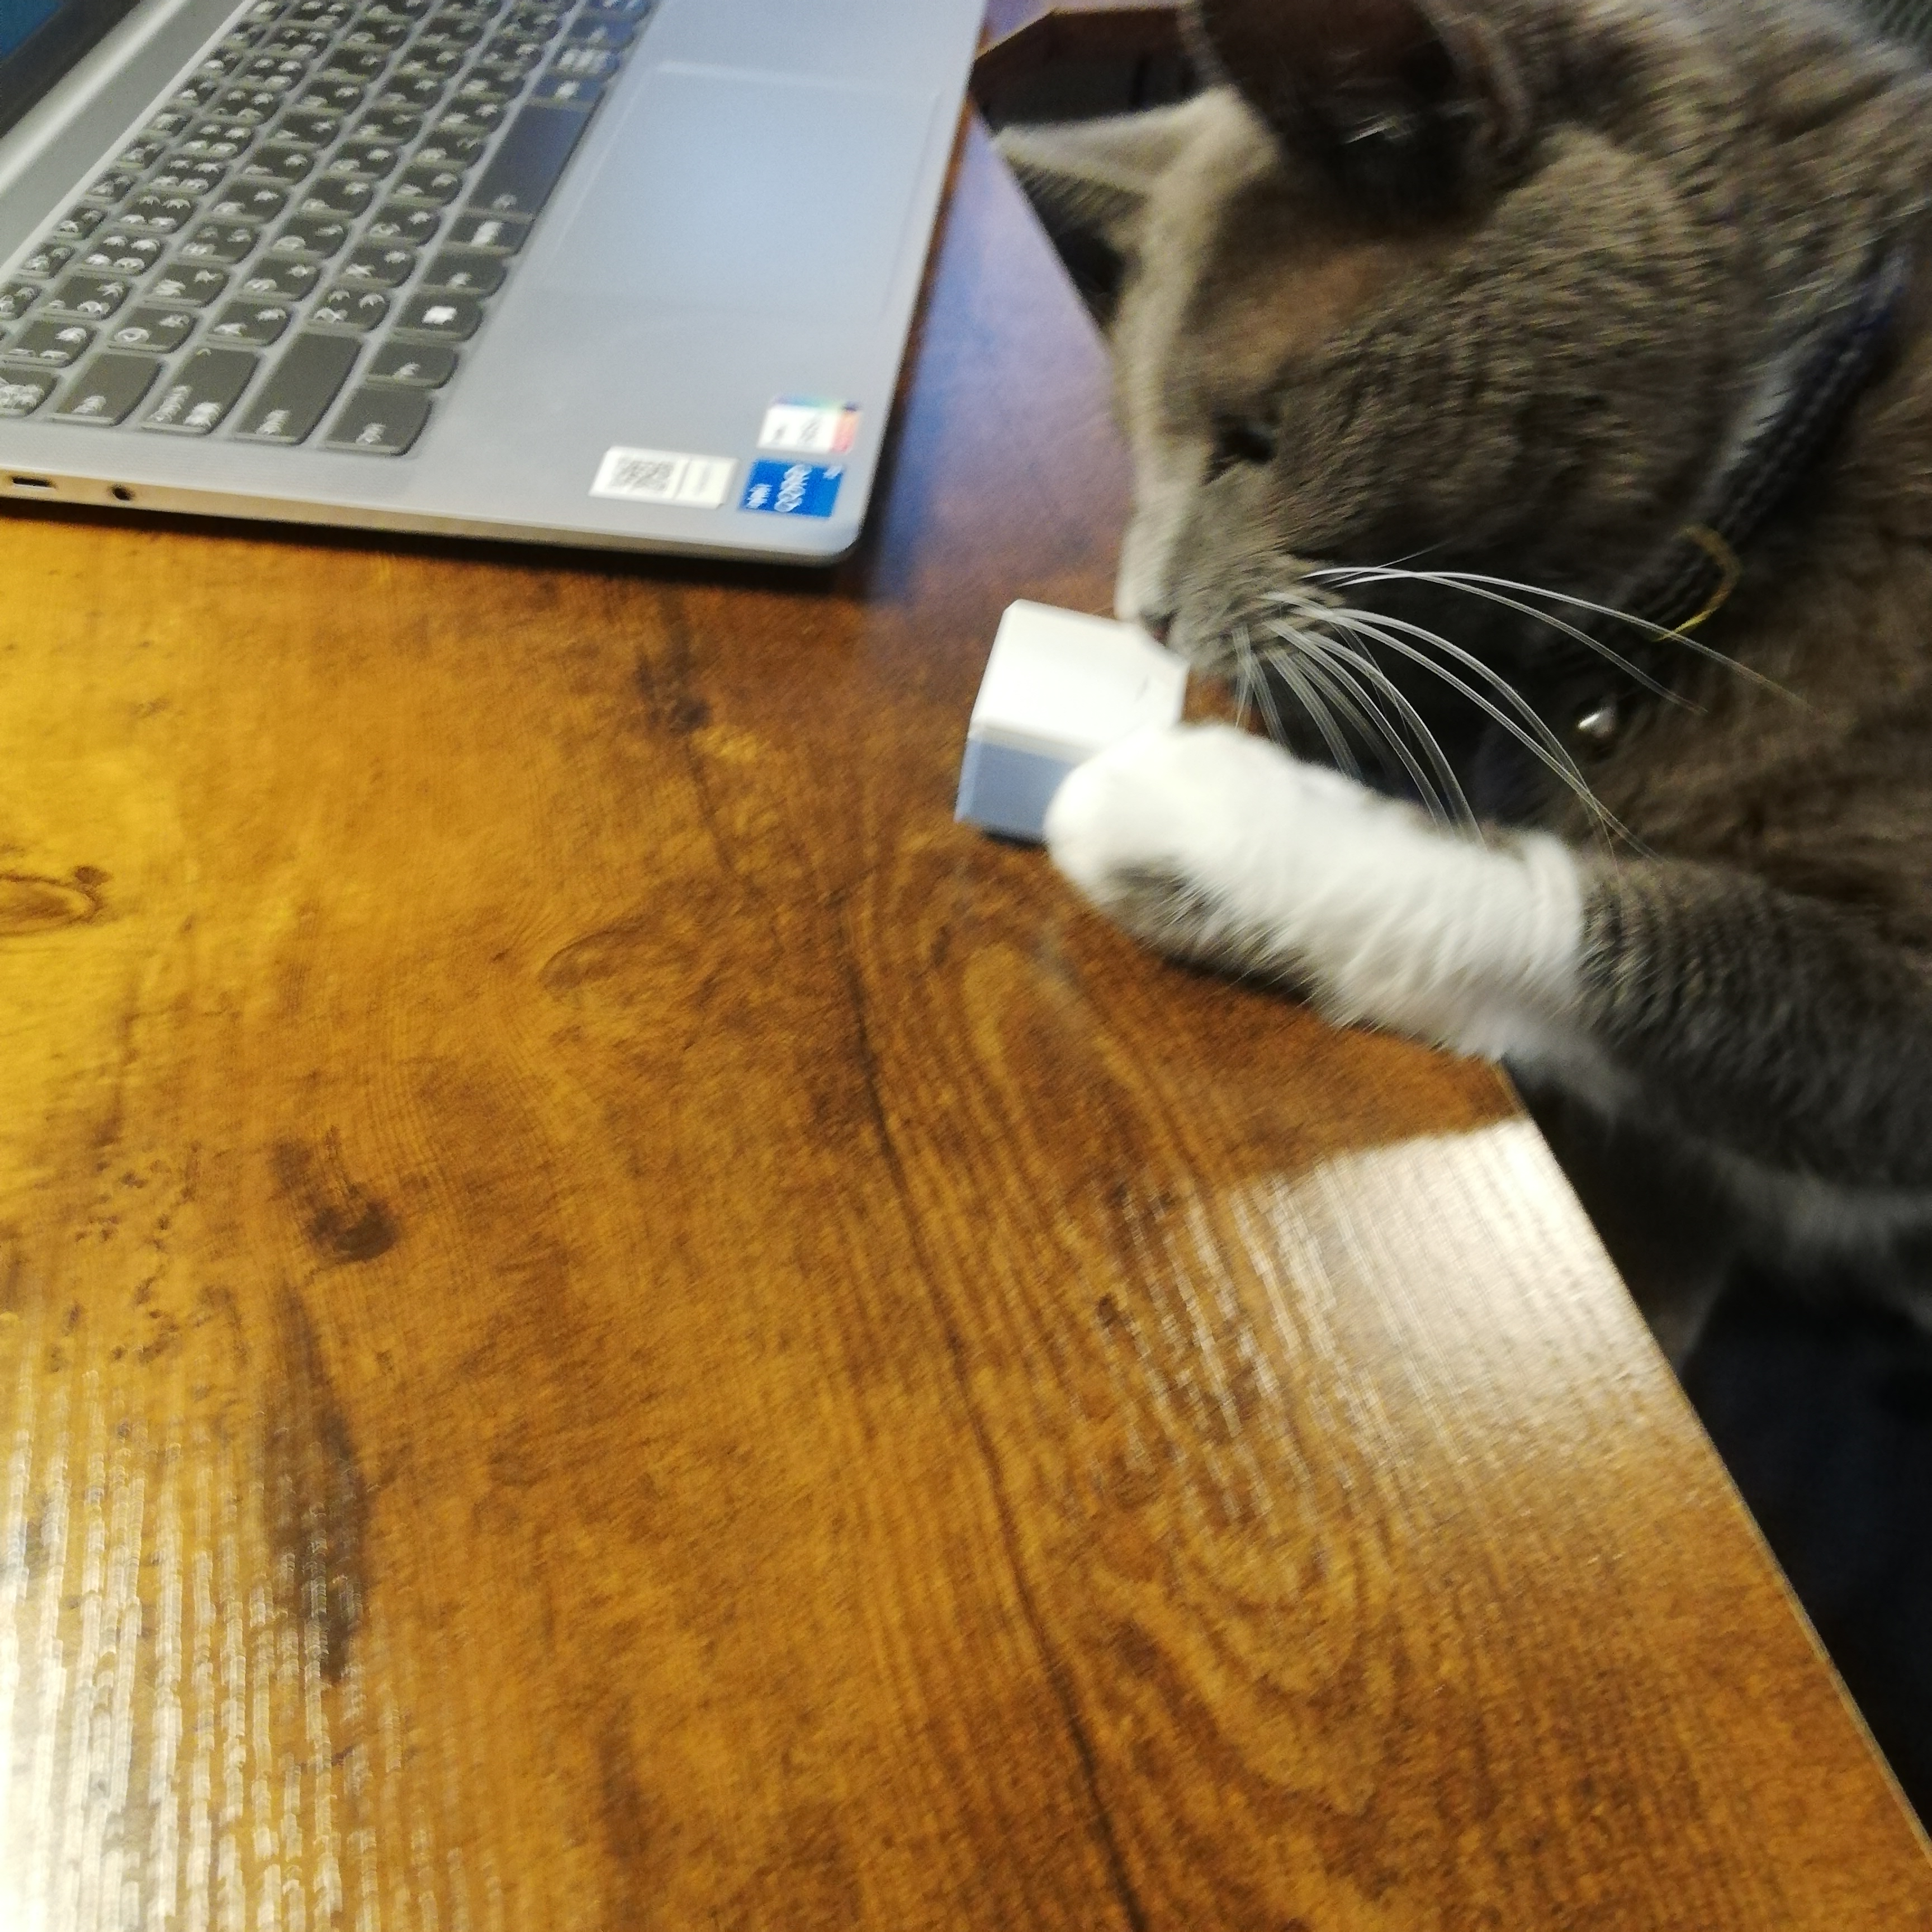
\includegraphics[width=0.9\textwidth]{resources/cat_after.jpg}
    \end{minipage}     &
    \begin{minipage}[c]{0.15\textwidth}
      \centering
      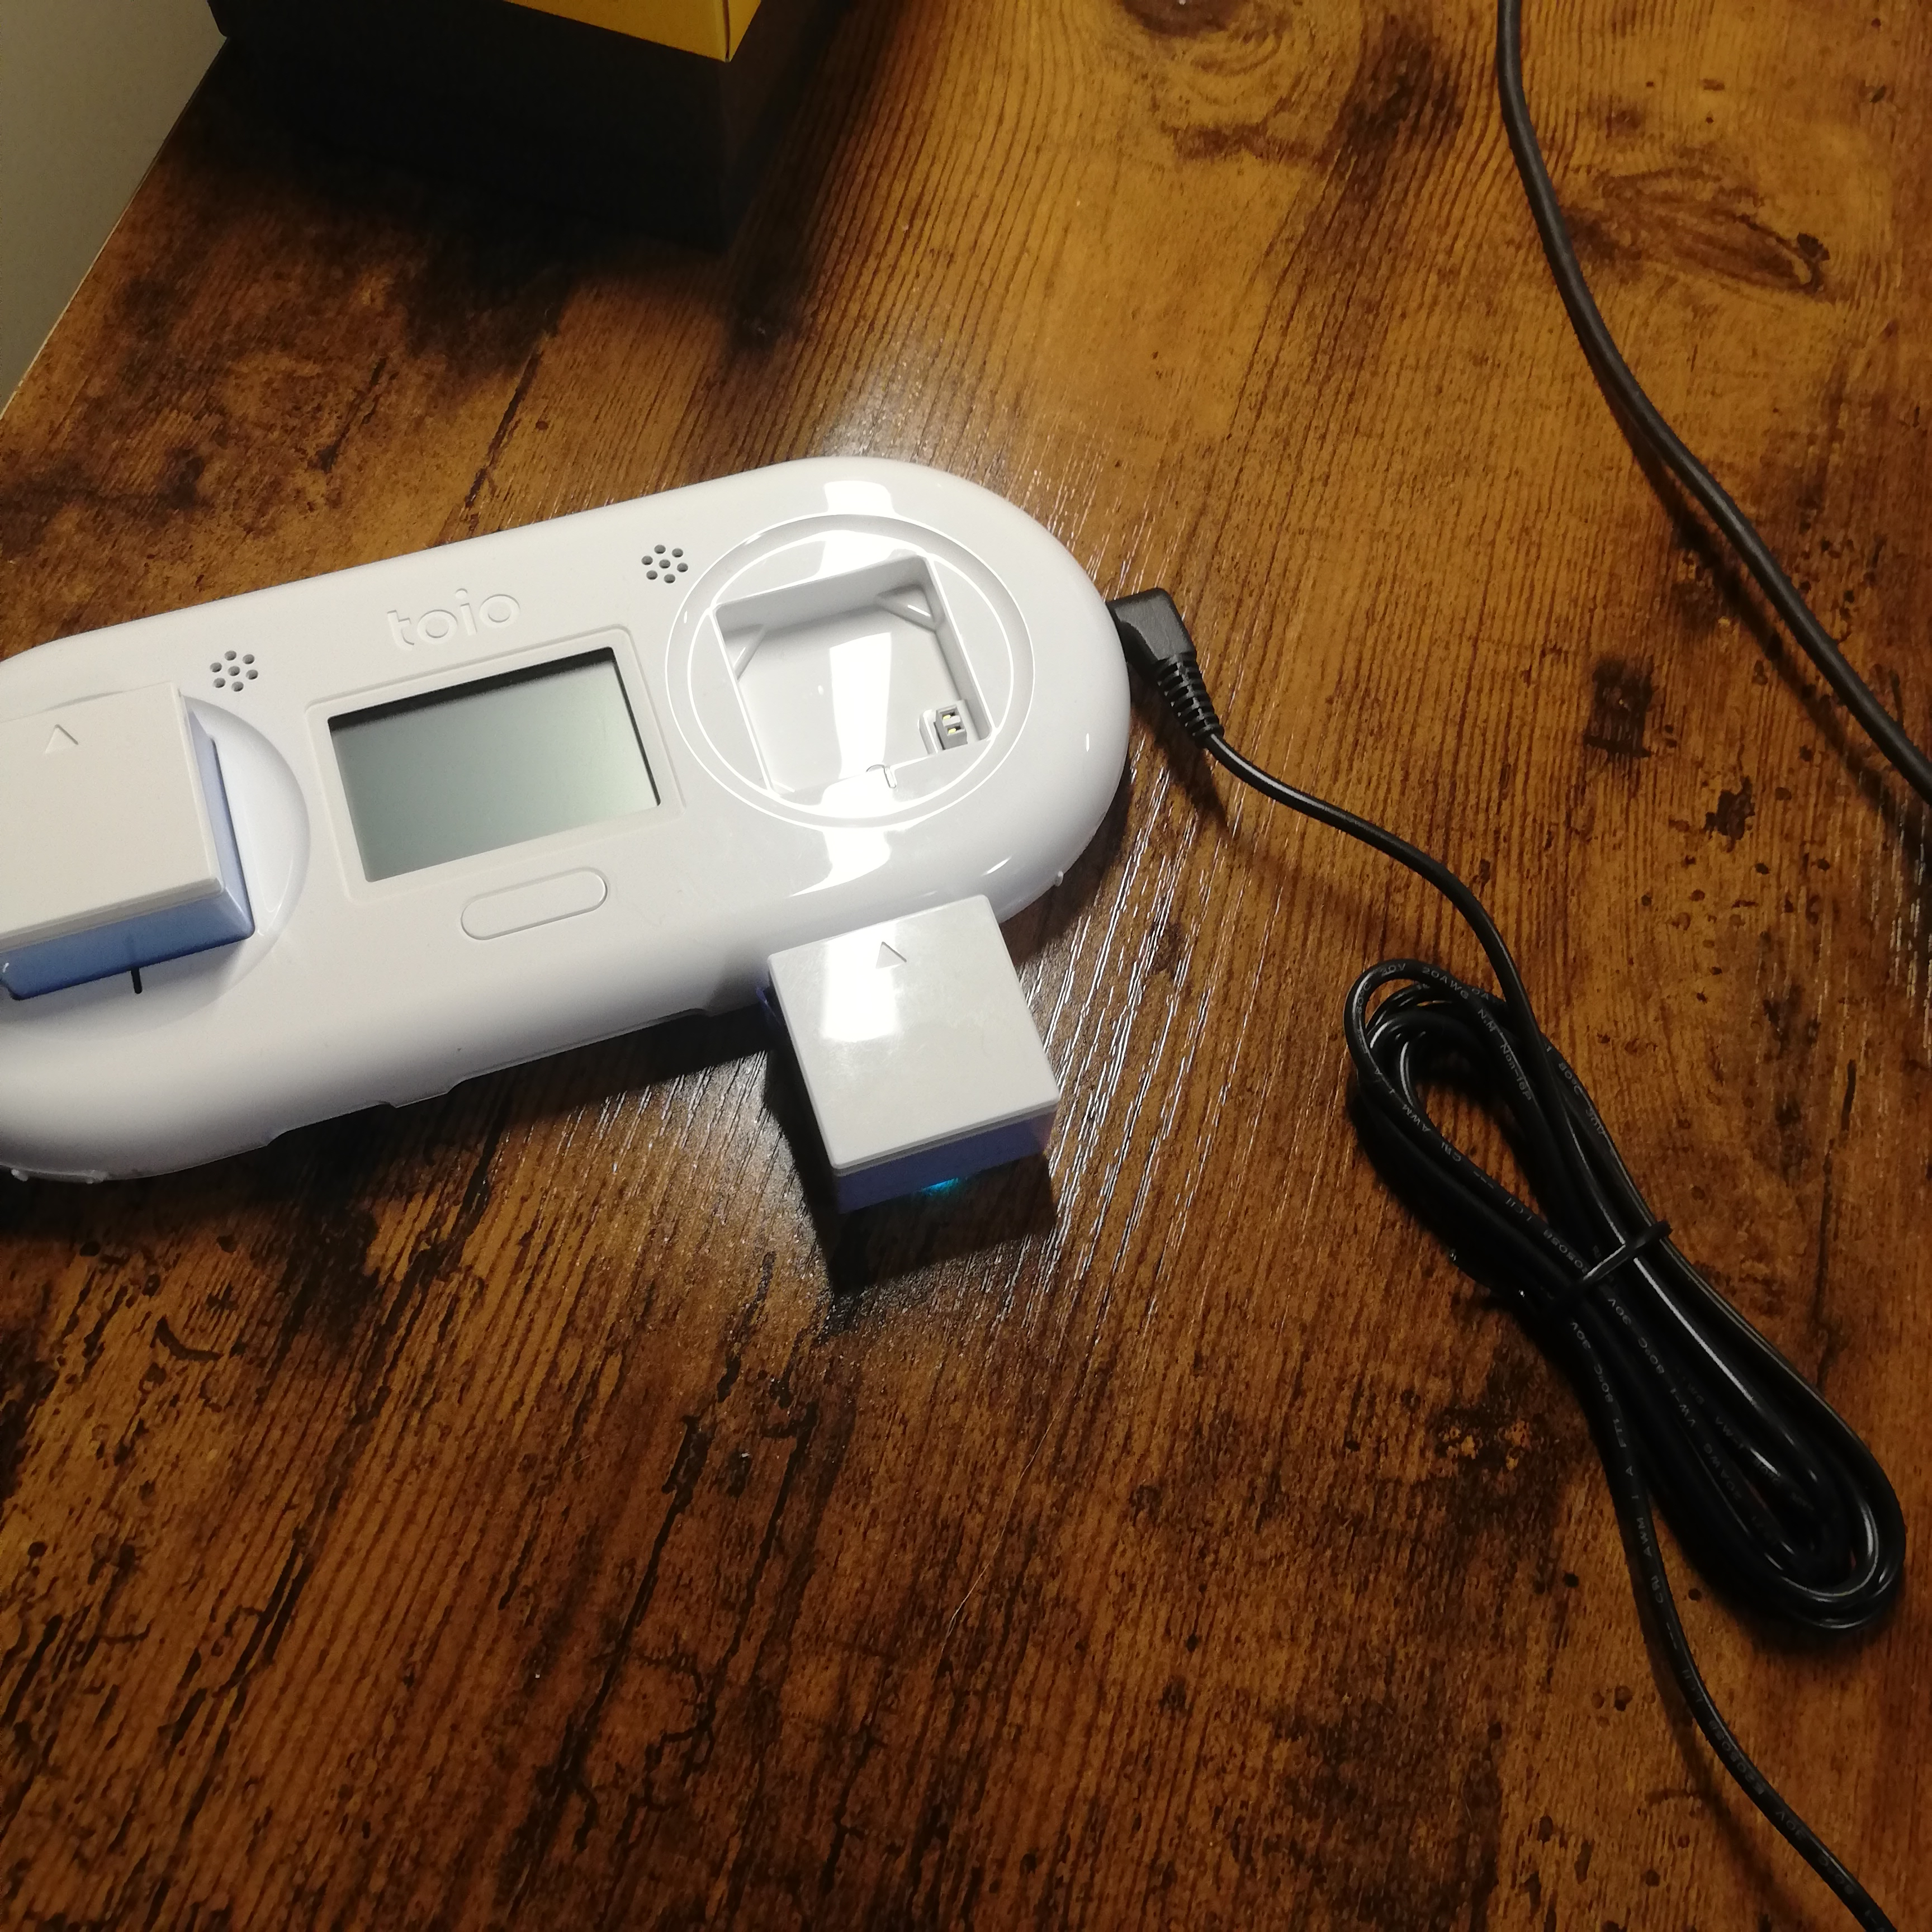
\includegraphics[width=0.9\textwidth]{resources/doc_after.jpg}
    \end{minipage}     &
    \begin{minipage}[c]{0.15\textwidth}
      \centering
      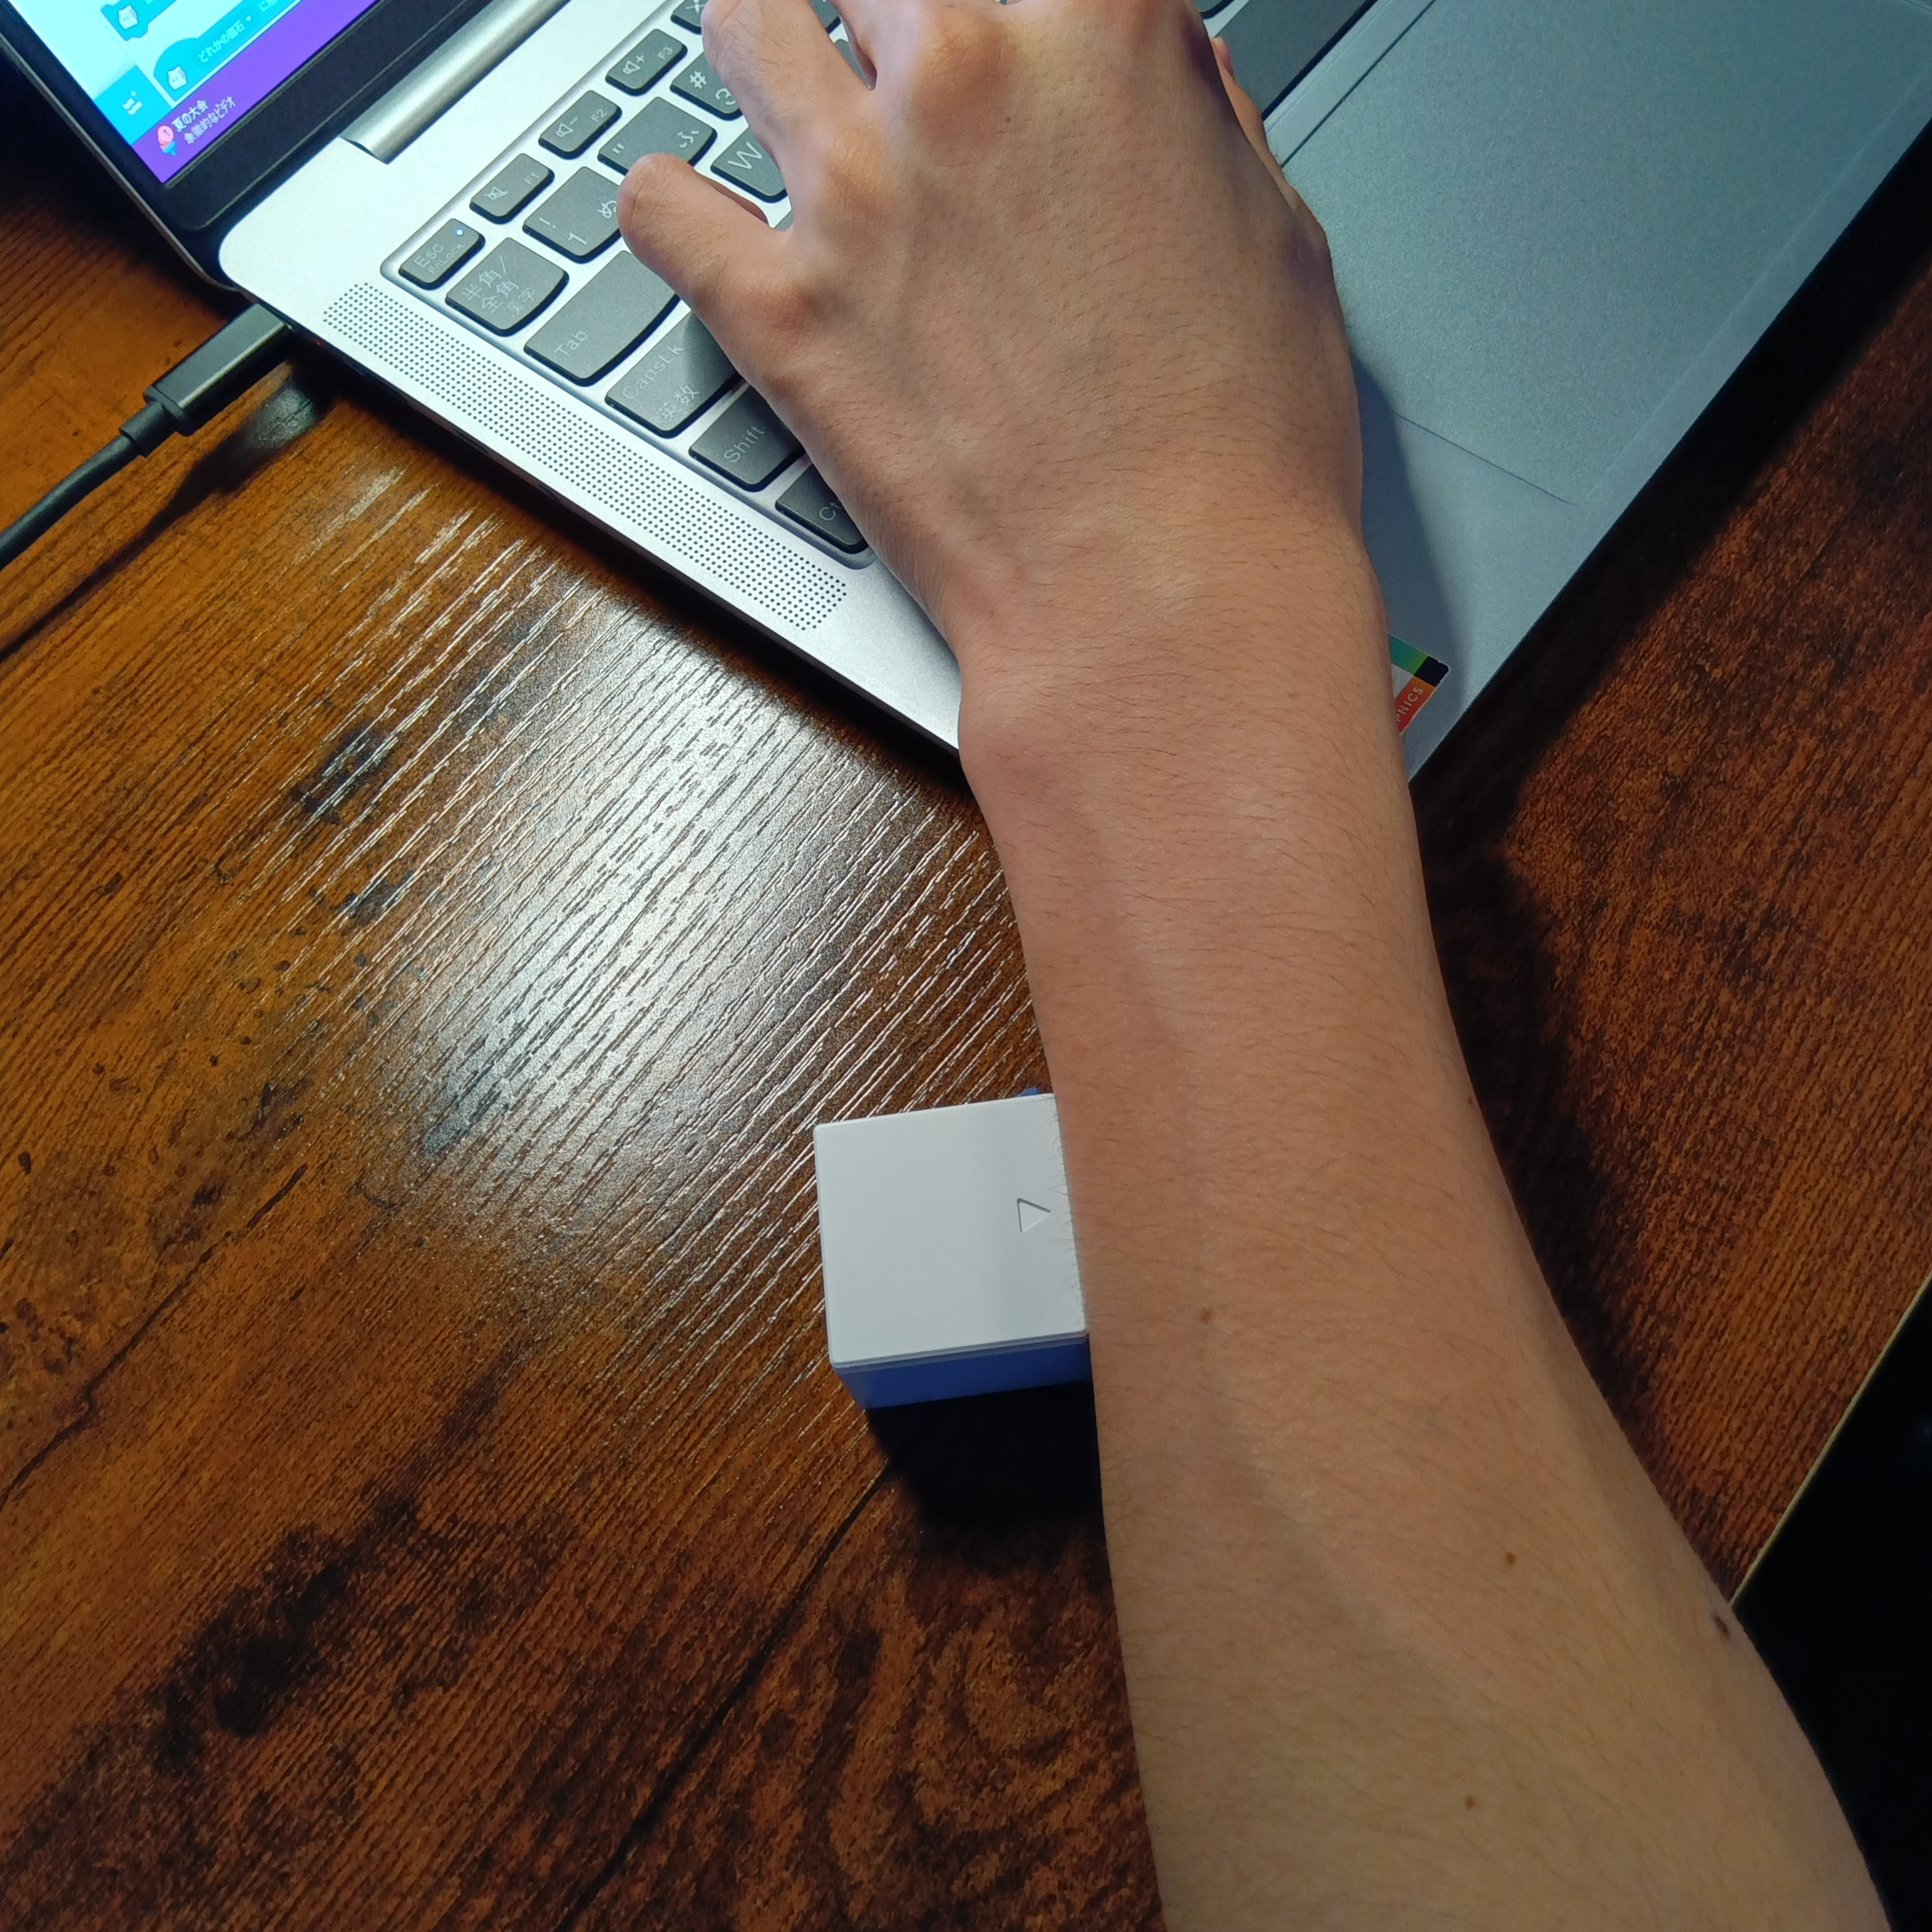
\includegraphics[width=0.9\textwidth]{resources/pet_after.jpg}
    \end{minipage}
    \\ \hline
  \end{tabular}
  \caption{仮置き}
\end{figure*}

\section{システムの制約と展望}
本システムは,Bluetooth通信を用いているため,屋内での使用を前提とし,通信可能な範囲内での動作に限られる.また,評価対象は基準が明確で計測可能なものに限定される.

今後の展開として,ロボット間の協調動作の実装や,より正確な環境評価のためのセンシング手法の改善が考えられる.さらに,異なるセンサーやロボットを組み合わせることで,新たなユーザー体験の創出も期待できる.

\section{おわりに}
本研究では,環境データを他者の視点から評価し,ロボットの身体的動作を通じて表現するシステムを開発した.M5StickCとtoioを用いたプロトタイプシステムの実装により,他者にとっての快・不快を直感的に理解できるインタフェースを実現した.特に,『弱いロボット』の概念を取り入れることで,ユーザーを自然にシステムフローに組み込むことができた.

今後は,より多様な他者の表現や,ロボット同士の協調動作の実装など,システムの拡張を進めていく.

%  ----- 参考文献 -----
% 参考文献リストの「参考文献」のスタイル
\renewcommand{\refname}{ 参考文献}
\bibliography{ref}
\bibliographystyle{junsrt}
\end{document}
